\subsection{Reasoning transfer in CLEVR-CoGenT}
\label{sec:reasoning-clevr}
In the following we have relied on the CoGent-A variant only.
Using the question groups (categories) defined by the authors, we reorganized training and testing splits with the goal of measuring whether mastering reasoning for one group can help with learning of the other.

\begin{figure}[htbp]
	\centering
	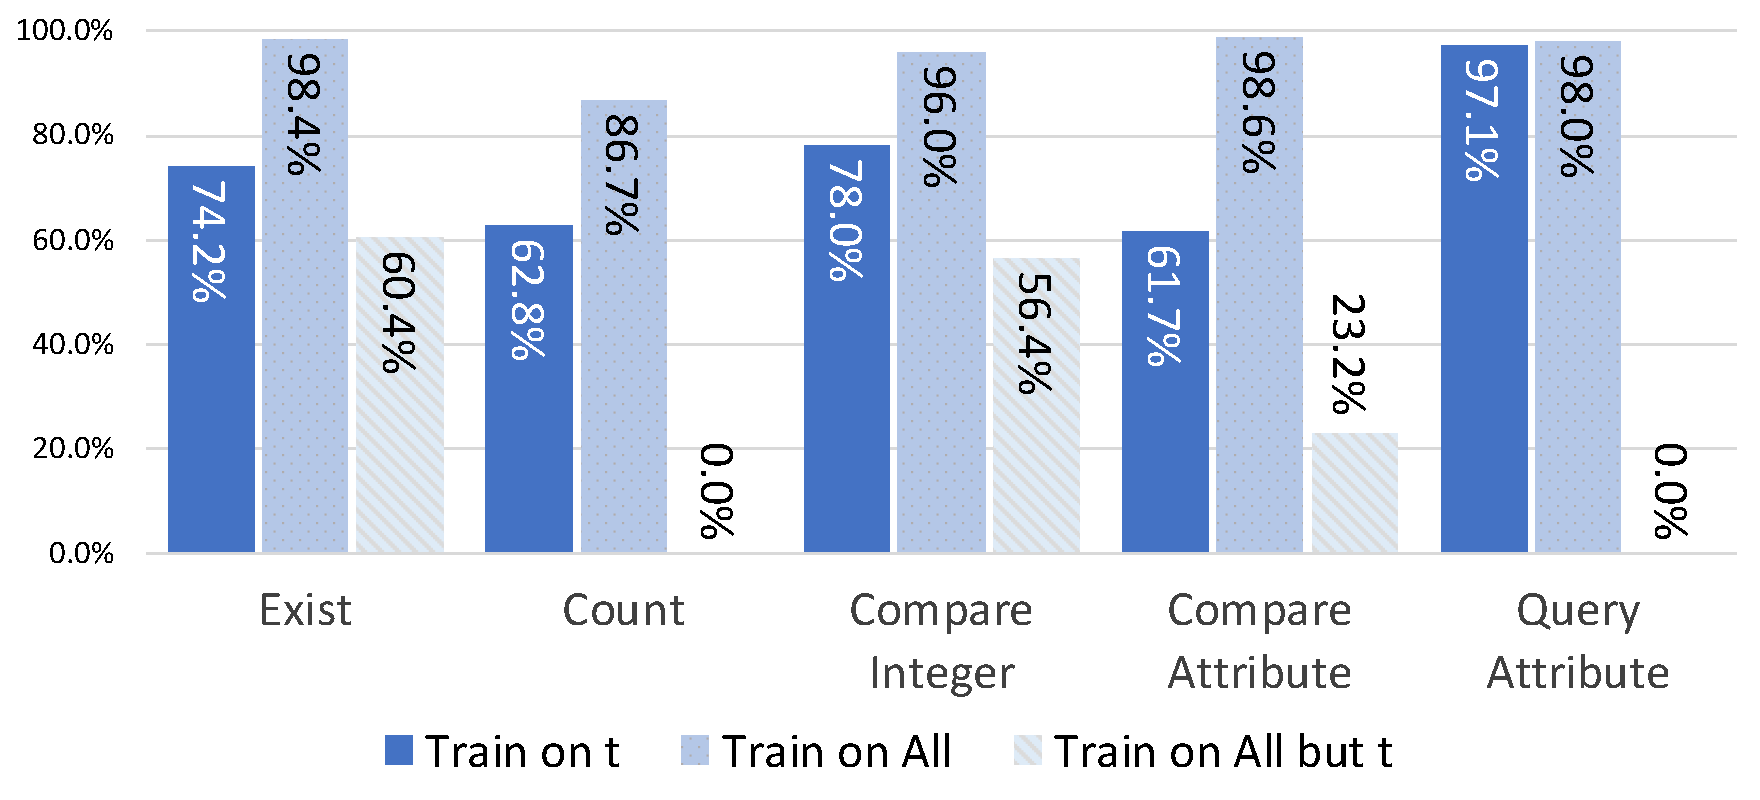
\includegraphics[width=\columnwidth]{../img/plots/cogent_reasoning_transfer.pdf}
	\caption{Accuracies of SAMNet when testing its reasoning transfer capabilities on the CoGenT-A variant.}
	\label{fig:cogent_reasoning_transfer}
\end{figure}

First we have trained a single SAMNet model and measured its accuracy on each of the task group $t$ separatelly.
Those results, indicated in \cref{fig:cogent_reasoning_transfer} as "Train on All", form baselines for the next two sets of experiments.

Next, we trained and tested 5 SAMNet instances, each on a single task group $t$.
Interestingly, we observe a significant accuracy drop in all task groups aside of the \textit{Query Attribute}.
We hypotesize this results from the fact that mastering visual grounding and recognizing object attributes (being the core of the latter task) is a necessary skill the system needed by the other tasks.
Thus training on \textit{Query Attribute} helps others, whereas without any training on that particular group the system struggles with developing such a skill.

Finally, we trained 5 SAMNet instances in the extreme reasoning transfer setup: for each task group $t$ we trained a single instance on all tasks but $t$, and next tested its performance on $t$ only.
As expected, this setup appeared to be difficult to deal with, observing severe performance drops, with accuracy of \textit{Count} and \textit{QueryAttribute} dropping to zero.
The explanation is that these categories expect  answers (digits 0-9, names of attributes) that do not overlap with answers in the other groups (binary yes/no), thus the model cannot predict these labels on in a zero-shot transfer.

%Besides, the zero accuracy on \textit{Count} can also be explained by the fact that it results from the need of totally different reasoning leading to the answer.
%The \textit{QueryAttribute} latter is more interesting, as when mastering e.g.  \textit{Exist} of  \textit{CompareAttribute} the model \textit{had} to develop some kind of understanding object attributes.
%Still, this result once again suggests that the model learned joint representation of object attributes and struggle with disentangling them without being explicitly trained on task facilitationg that (like the  \textit{QueryAttribute}).



% An additional set of experiments, for which results are available in the supplementary material, fine-tune the model trained on all tasks on each task $t$ respectively.
%Fine-tuning did not demonstrate a clear benefit (except for \textit{Count}, where the accuracy increased by 1.5 pt) without hurting performance on the other tasks. Nevertheless, these experiments leave open the possibility that joint training of tasks may potentially benefit from using weighted sampling towards the tail end with more emphasis on samples from less performing task groups, similar to~\cite{guo2018dynamic, kendall2018multi}.

\subsection{Reasoning transfer in COG}
\label{sec:reasoning-cog}

\begin{figure}[htbp]
	\centering
	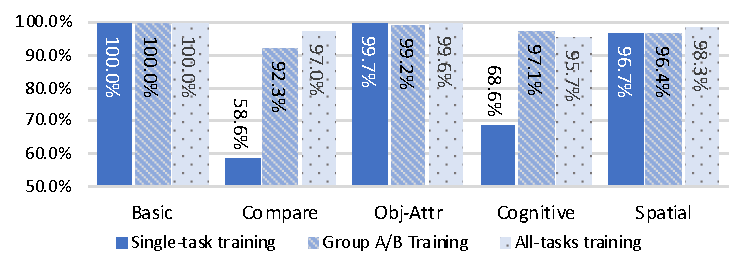
\includegraphics[width=\columnwidth]{../img/plots/cog_reasoning_transfer.pdf}
	\caption{Accuracies of SAMNet when testing its reasoning transfer capabilities on the Canonical variant of COG.}
	\label{fig:COG-reasoning-results}
\end{figure}\vspace{2pt}

Reusing the task hierarchy in \cref{fig:task-groups}, we conduct the following experiments using the Canonical variant of COG to study whether reasoning transfer learning was effective in leveraging information gained by training a task family at a higher level
of the hierarchy:
 \begin{itemize}
 	\compresslist
	\item Train and test SAMNet on each of the 5 task groups at the lowest level of the hierarchy (Single-task training);
	\item Jointly train on:
	\begin{itemize}
		\item \textbf{Group A} and test on each task from the lowest groups (i.e. \textbf{Basic}, \textbf{Obj-Attr} and \textbf{Compare}) separately;
		\item \textbf{Group B} and test separately on \textbf{Spatial} and \textbf{Cognitive};
	\end{itemize}
	\item As a baseline, we compared the above results to the earlier experiment shown in~\cref{fig:samnet_cog_detailed}, which can be viewed as training jointly on \textbf{All} and testing on each group at the leaf level separately (All-task training).
\end{itemize}

The results of these experiments are shown in~\cref{fig:COG-reasoning-results}.

First, notice that for each of the \textbf{Basic} and \textbf{Obj-Attr} task families, the accuracy is near-perfect in all cases, suggesting that each contains the most primitive tasks and therefore do not benefit from training with other task families.
With \textbf{Spatial}, we see a small improvement showing that there is some benefit due to joint training with other task families.
Two groups that demonstrated a huge improvement of more than 25 points are \textbf{Compare} and \textbf{Cognitive}.
The former saw an accuracy jump from 58.6\% by training on samples from that family alone
to 97.0\% when training on all samples. To further emphasize this behavior, notice that
just joining \textbf{Compare} with \textbf{Obj-Attr} and \textbf{Basic} already causes a significant accuracy jump to 92.3\%.
In hindsight, this is not surprising, as the questions in \textbf{Compare} are composed
of fragments of questions given by \textbf{Basic} and \textbf{Obj-Attr}, and therefore can leverage the reasoning strategies developed there to reason about questions in \textbf{Compare}.
Lastly, for the \textbf{Spatial} family, we again see the benefits of joint training with all questions (68.6\% to 95.7\%) but in this case there
is a slight loss incurred by including everything. As seen in the figure, just jointly training with \textbf{Spatial} alone is sufficient to get a boost in accuracy (97.1\%). To summarize, while joint training helps, one needs to determine how much of correlation is present with the other tasks.
